\documentclass[12pt,a4paper]{article}

\usepackage{graphicx}
\usepackage{amsmath}
\usepackage{caption}
\usepackage{float}
\usepackage{geometry}

\geometry{margin=1in}

\title{Plots}
\author{}
\date{}

\begin{document}

\maketitle

\begin{figure}[H]
\centering
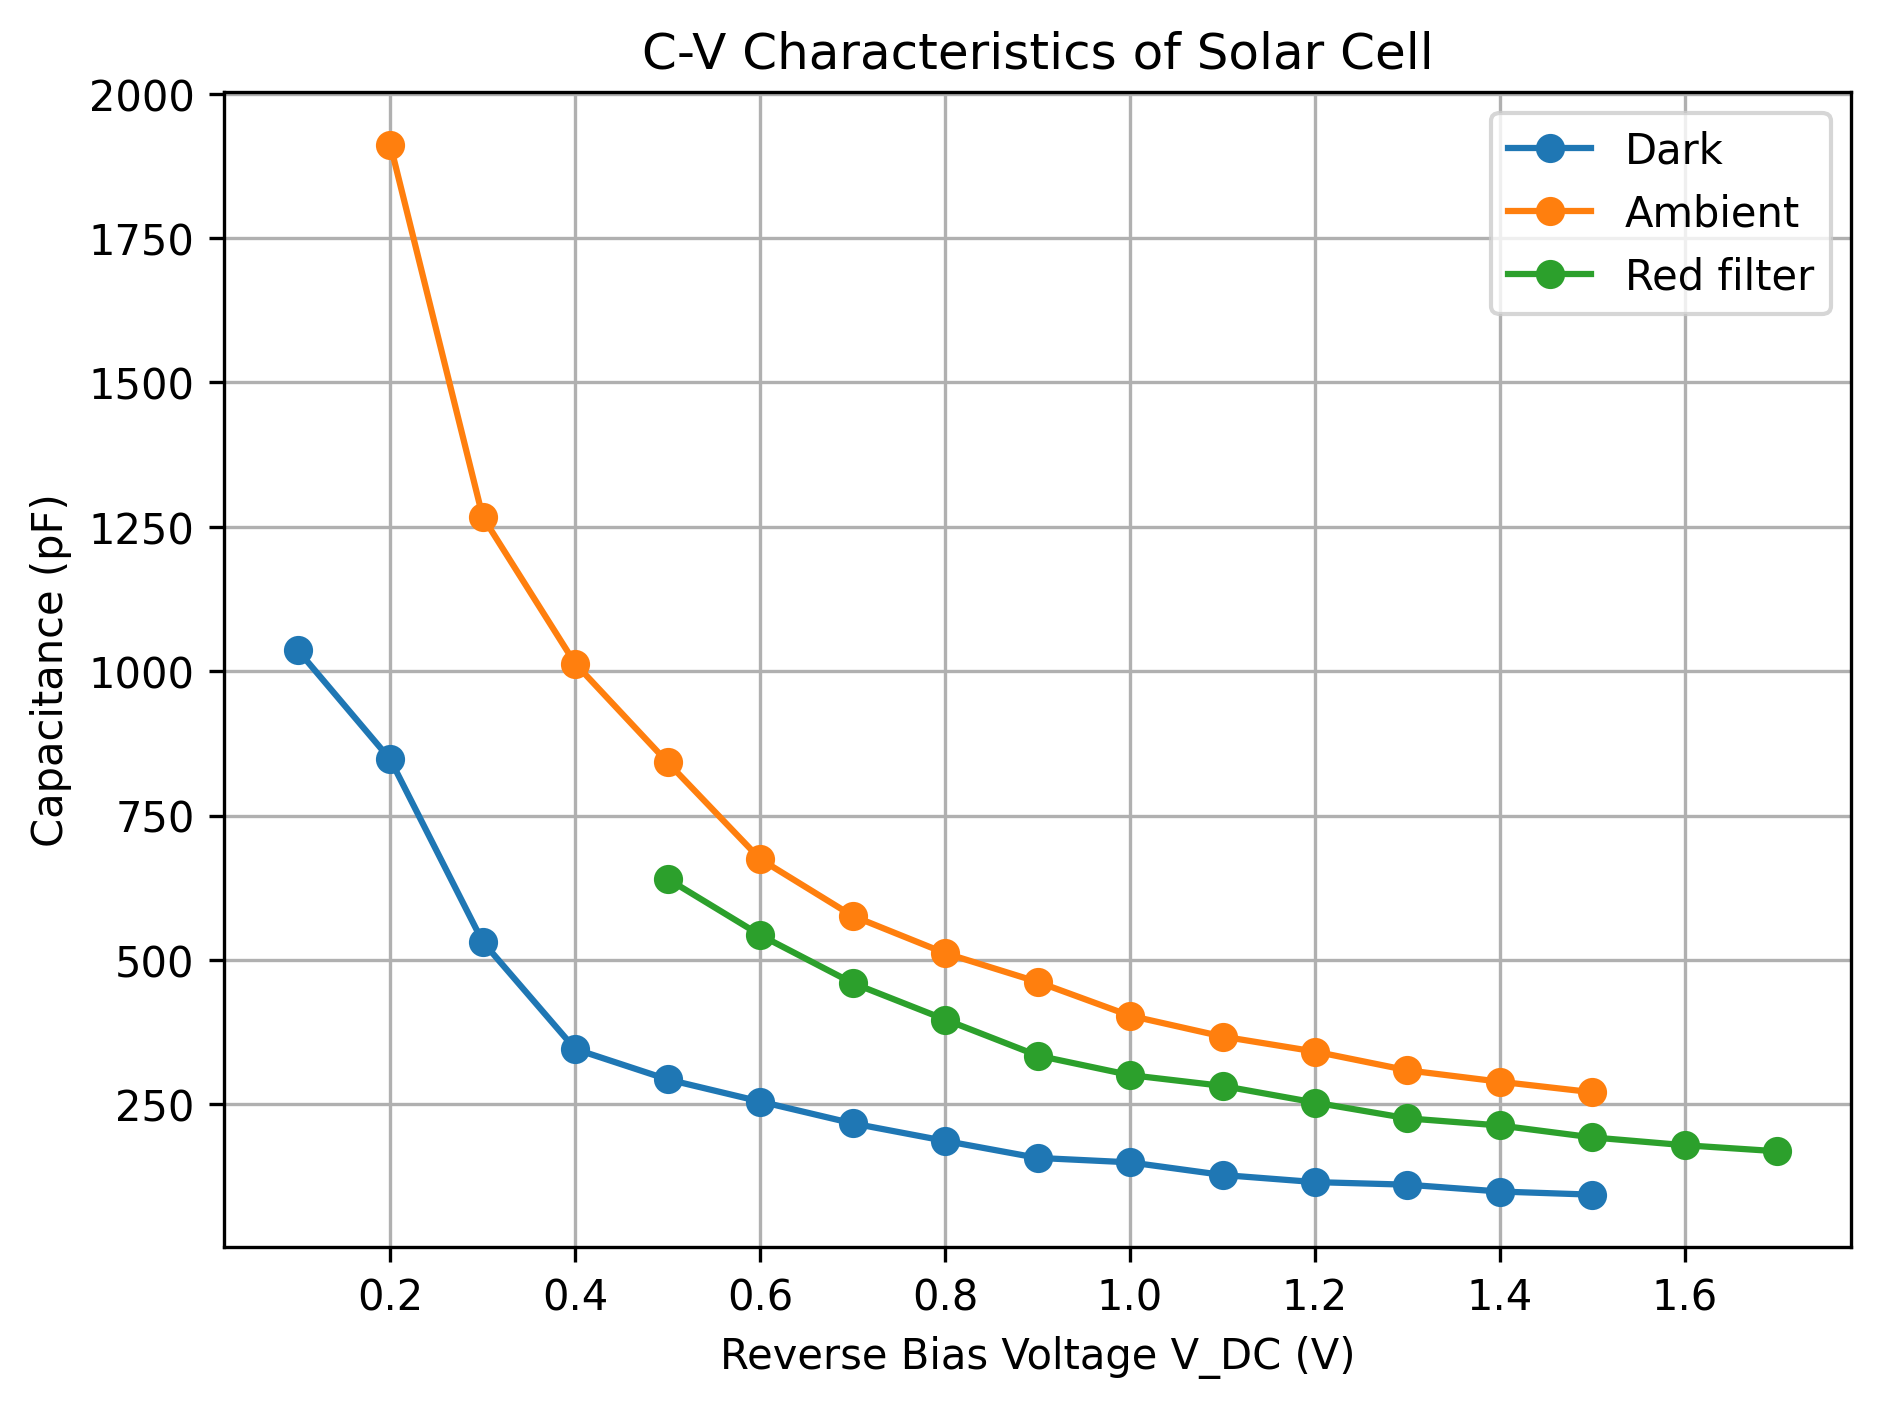
\includegraphics[width=0.8\textwidth]{CV_characteristics.png}
\caption{C–V characteristics of the solar cell under different illumination conditions (dark, ambient light, and red filter). The capacitance decreases as the reverse bias voltage increases due to the widening of the depletion region.}
\label{fig:cv}
\end{figure}


\begin{figure}[H]
\centering
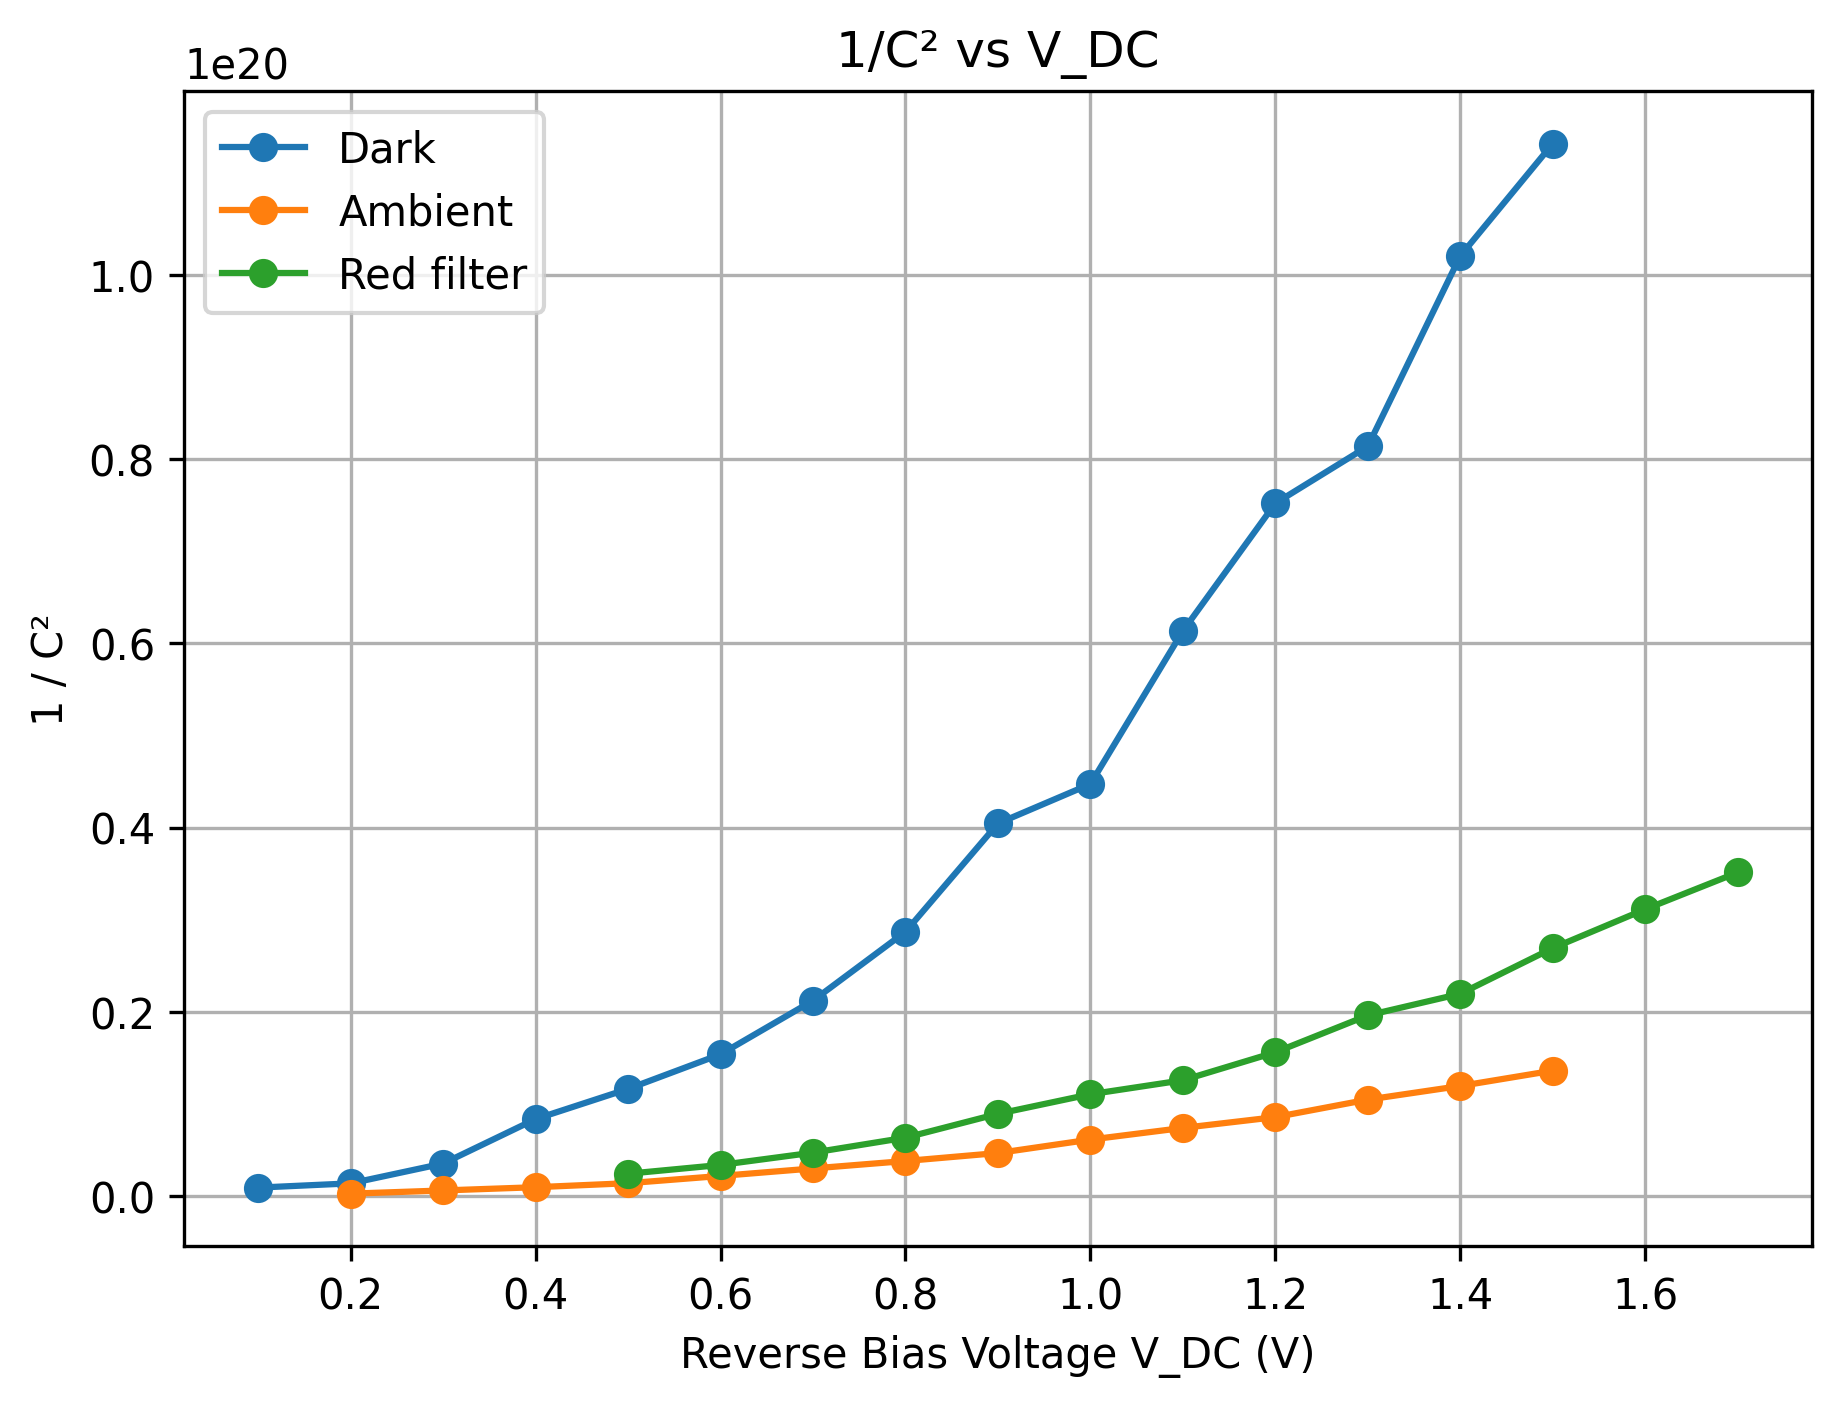
\includegraphics[width=0.8\textwidth]{inverseC2_vs_V.png}
\caption{Plot of $1/C^2$ versus reverse bias voltage $V_{DC}$ under dark, ambient light, and red filter conditions. This plot can be used to estimate the built-in potential and doping concentration of the junction.}
\label{fig:invC2}
\end{figure}




\end{document}
